\documentclass[a4paper,12pt]{article}
\usepackage[utf8]{inputenc}
\usepackage[francais]{babel}
\usepackage{listings}
\usepackage{textcomp}
\usepackage[usenames,dvipsnames]{xcolor}
\usepackage{graphicx}
\usepackage{hyperref}
\usepackage{chngcntr}
\usepackage{amsmath}

% Configuration des liens
\hypersetup{
    colorlinks,
    citecolor=black,
    filecolor=black,
    linkcolor=black,
    urlcolor=black
}

% Configuration des blocs de code
\lstset {
upquote=true,
columns=flexible,
stringstyle=\ttfamily,
aboveskip=\topsep,
belowskip=\topsep,
breaklines,
basicstyle=\small,
breakindent=1.5em,
showstringspaces=false,
numbers=left,
frame=shadowbox,
numberstyle=\tiny\color{gray},
rulecolor=\color{gray},
language=php,
commentstyle=\color{BrickRed}
}

% Réinitialisation du compteur de sections pour chaque partie
\counterwithin*{section}{part}

% Espace entre les paragraphes
\setlength{\parskip}{10pt}

% Page de garde
\title{\textbf{\texttt{Dojoctylo}} - Rapport de projet}
\author{\textsc{Baptiste Vannesson}}
\date{\textit{\today}}

\begin{document}
\maketitle
\begin{figure}[!h]
\begin{center}

\includegraphics[scale=0.3]{taipingu-clavier.png}
\end{center}
\end{figure}

\begin{center}
  \url{http://21411850.users.info.unicaen.fr/dojoctylo/site}
\end{center}

\newpage
\tableofcontents
\newpage
\listoffigures
\newpage

% \begin{abstract}
% \end{abstract}

% ==========================================================================
% ============================== Introduction ==============================
% ==========================================================================

\part*{Introduction}

De nos jours, c'est presque un truisme de dire que les claviers sont partout. En effet, au travail comme à la maison, il est fort probable que vous passiez un temps non négligeable à utiliser un ordinateur. Le clavier s'avère donc indispensable.

Mais en dépit de cette réalité, la plupart des gens n'utilisent pas le clavier correctement, et certains sont même franchement maladroits avec cet outil... On dit souvent que bon nombre des problèmes informatiques sont liés à l'inévitable \og~interface chaise-clavier~\fg. Or ceci n'est guère étonnant si la maîtrise des outils du quotidien demeure entre les mains d'une poignée de geeks. L'informatique s'est largement démocratisée ces dernières décennies, mais pas forcément le savoir-faire élémentaire qui l'accompagne. C'est donc tout naturellement ici qu'intervient Dojoctylo~: le site web qui va faire de vous un ninja du clavier~!

Dans ce rapport, nous allons expliciter tous les aspects de ce projet, en commençant par le contexte. Nous y aborderons les éléments qui justifient l'intérêt de ce projet, et nous regarderons ce qui se fait déjà dans l'espace numérique à ce propos. Ensuite nous présenterons le site avec une vision fonctionnelle. Ce sera notamment l'occasion pour le lecteur de bien cerner ce qu'offre Dojoctylo en matière d'apprentissage, mais aussi de divertissement. Enfin nous parlerons bien sûr de la dimension technique inhérente au développement, sans oublier les perspectives d'évolution à plus ou moins long terme.

\newpage

% ==========================================================================
% ============================== I. Contexte ===============================
% ==========================================================================

\part{Contexte}

Un projet, un contexte... Dojoctylo ne sort pas d'un chapeau~: il s'inscrit dans un environnement tangible. Dans un premier temps, nous allons présenter quelques constats empiriques qui démontrent tout l'intérêt d'un tel site web. Dans un deuxième temps, nous ferons une rapide étude de marché en mettant en exergue les points forts et les points faibles de la \og~concurrence~\fg.

\section{Constats empiriques}

Le développement de Dojoctylo s'appuie sur quatre grands constats empiriques~: l'omniprésence du clavier dans nos sociétés contemporaines, le culte paradoxal de l'improductivité, les problèmes de santé (TMS), et une concurrence limitée sur le segment de la dactylographie.

\subsection{L'omniprésence du clavier}

C'est un fait~: nul ne peut aujourd'hui échapper aux claviers, à moins d'être atteint d'une technophobie irrépressible ou de vivre avec très peu de moyens dans un endroit isolé. Qu'ils soient physiques, tactiles, ou holographiques, les claviers font partie de notre quotidien et représentent l'interface de base qui nous permet d'interagir avec les dispositifs électroniques qui nous entourent.

Certains procédés, comme la reconnaissance vocale, existent déjà et constituent une réelle alternative à l'utilisation du clavier. Cependant, cette technologie en est encore au stade embryonnaire en ce qu'elle est loin d'offrir la précision d'une saisie manuelle. Qui ne s'est jamais amusé avec un logiciel de reconnaissance vocale comprenant la plupart des questions de travers~?

À l'heure actuelle, le clavier reste donc la référence, quel que soit le support. Ceci est par conséquent une raison suffisante pour apprendre à s'en servir. Il est d'ailleurs étonnant de constater que l'écriture manuelle est considérée comme un apprentissage fondamental, tandis que l'enseignement de la frappe au clavier reste très largement secondaire, voire inexistant, à l'école. Un joli paradoxe quand on sait que beaucoup de personnes passent plus de temps à taper sur un clavier qu'avec un stylo en main...

\subsection{Le culte paradoxal de l'improductivité}

La dactylographie est une discipline apparue à la fin du XIX\ieme{} siècle, dans un contexte de révolution industrielle. Elle est évidemment concomitante au développement des machines à écrire. Initialement, la dactylographie était un métier à part entière, mais depuis l'apparition des ordinateurs personnels, la saisie de textes au clavier est déléguée majoritairement aux secrétaires.

Ce bref historique a le mérite de nous montrer que la dactylographie revêt aussi une dimension sociale. Si autant d'individus, même dans les plus hautes sphères intellectuelles, ne maîtrisent pas le clavier, c'est peut-être aussi parce que la maladresse avec cet outil est tacitement et involontairement valorisée. La dactylographie est la discipline du copiste, c'est-à-dire celui qui reproduit les documents, sans forcément prendre la peine de penser par lui-même. On attend avant tout du dactylographe qu'il reproduise rapidement et fidèlement des documents écrits, un peu à la manière d'une machine.

Cependant, cette vision des choses est profondément désuète, et il est temps de changer les mentalités. La dactylographie est avant tout une discipline au service de la productivité. Une fois maîtrisée, elle permet de se concentrer sur l'essence du contenu à taper plutôt que sur les caractères qui le constituent. Bien loin d'être une simple pratique de copiste, la dactylographie a pour but d'automatiser le dérisoire pour que toute l'attention du pratiquant soit finalement captée par l'essentiel.

\subsection{Les troubles musculosquelettiques (TMS)}

Au-delà des questions ayant trait à la productivité, la dactylographie est aussi un rempart aux problèmes de santé. Aujourd'hui, les troubles musculosquelettiques représentent la cause principale des maladies professionnelles, et il va de soi que le clavier n'y est pas complètement étranger. En effet, un usage quotidien et prolongé du clavier peut provoquer des douleurs si l'usage qui en est fait ne respecte pas les rudiments de l'ergonomie du poste de travail. Les douleurs se situent généralement au niveau de la main, et plus généralement du bras (poignet, coude, épaule)~; le cas typique étant le syndrome du canal carpien. Le cou n'est pas non plus exclu car il est particulièrement sollicité lorsque l'utilisateur fait des allers-retours constants entre l'écran et le clavier.

La dactylographie, autrement dit la frappe à l'aveugle et à dix doigts, permet donc de se prémunir contre les problèmes de santé en apportant à celui qui la pratique un réel confort de travail. L'utilisation de matériel adapté est aussi une condition nécessaire, bien que non suffisante.

\subsection{Une concurrence limitée sur le segment de la dactylographie}

Si l'on observe quelque peu le paysage concurrentiel sur le terrain de la dactylographie, en France, force est d'admettre que tout cela n'est pas bien féroce... On trouve naturellement quelques sites qui permettent de pratiquer la saisie du français, mais peu mettent réellement l'accent sur l'apprentissage technique des dispositions francophones, rares sont ceux qui ont une interface aboutie, et en plus de cela les sites sont souvent étrangers.
Il y a bien quelques concurrents sérieux qui proposent des solutions d'apprentissage innovantes, ludiques, et presque professionnelles, mais ce sont souvent des sites en anglais qui proposent d'apprendre le QWERTY. Pas très intéressant pour les Français qui ne sont pas très à l'aise avec la langue de Shakespeare et qui passent leur vie sur un clavier AZERTY...

\section{Étude de l'existant}

La concurrence sur le segment de la dactylographie n'est pas très intense. Malgré tout, certains acteurs sérieux sont déjà bien implantés. Nous verrons principalement ici ceux qui proposent d'apprendre à taper au clavier avec des textes en français. Nous ferons néanmoins une exception pour présenter un site uniquement anglophone, mais extrêmement intéressant dans son approche. Nous présenterons aussi brièvement des sites qui proposent quelque chose d'un peu différent~: la dactylographie pour programmeurs.

\subsection{Apprentissage de la dactylographie traditionnelle}

Nous allons voir dans cette partie quatre applications qui méritent largement d'être présentées~: Klavaro, 10FastFingers, Keyhero, et Nitro Type.

\subsubsection{Klavaro}

Klavaro est un logiciel libre pour apprendre la dactylographie. C'est un logiciel relativement sobre, mais très adapté pour celles et ceux qui souhaitent apprendre à bien taper au clavier. Klavaro gère de nombreuses langues et dispositions de clavier. Le logiciel propose quatre modes de pratique, faisant suite à une introduction au cours de laquelle les rudiments de la dactylographie sont brièvement expliqués. Ces modes sont les suivants~:

\begin{itemize}
 \item{\og~Cours de base (Première étape~: entraînement initial)~\fg}
 \item{\og~Adaptabilité (Entrainement avec touches aléatoires)~\fg}
 \item{\og~Vitesse (Entrainement avec mots aléatoires)~\fg}
 \item{\og~Fluidité (Entrainement avec des textes complets)~\fg}
\end{itemize}

Dans les cours de base, le logiciel se focalise sur des fragments de clavier, généralement des touches consécutives ou sur la même rangée, pour permettre à l'utilisateur de s'exercer sur des points précis. Au début, on retrouve le très classique \og~fj~\fg, mais le niveau est croissant.

L'exercice d'adaptabilité représente l'aboutissement des cours de base puisque l'objectif est ici de taper des séries de caractères aléatoires. Le tout n'a évidemment aucun sens, mais le but est de voir si on a bien mémorisé la position des touches sur l'ensemble du clavier.

Dans la logique des choses, vient ensuite l'exercice de vitesse. Ici, l'utilisateur doit taper le plus vite possible une longue série de mots générée aléatoirement par le programme. La touche de correction est désactivée pour vraiment se focaliser sur la vitesse.

Enfin, l'exercice le plus difficile~: celui de fluidité. Dans ce mode, l'utilisateur doit saisir le plus rapidement et précisément possible un texte donné. La fluidité, qui tient compte de toutes les accélérations et décélérations, doit être constante. La correction est disponible et l'utilisateur peut choisir le nombre de paragraphes (de 1 à 10). Pour valider l'exercice, le logiciel exige une précision supérieure à 97~\%, une vitesse d'au moins 50 mots par minute (MPM), et une fluidité minimale de 70~\%. En règle générale, c'est loin d'être simple de répondre simultanément à tous ces critères. L'exigence de fluidité est même contradictoire car un dactylographe qui tape vite et précisément n'est pas nécessairement un dactylographe constant dans sa frappe. Il faut savoir accélérer dans les passages faciles et ralentir dans les passages difficiles. Or ceci dépend beaucoup du texte.

En dehors des modes de pratique stricto sensu, Klavaro propose un suivi de la progression ainsi qu'une compétition déguisée, sous la forme d'un top 10. Malheureusement, ces fonctionnalités sont assez rudimentaires... À noter toutefois qu'il est possible d'ajouter ses propres textes, ce qui est plutôt pas mal pour ajouter un peu de piment dans l'utilisation de ce logiciel.

\begin{figure}[!h]
\begin{center}
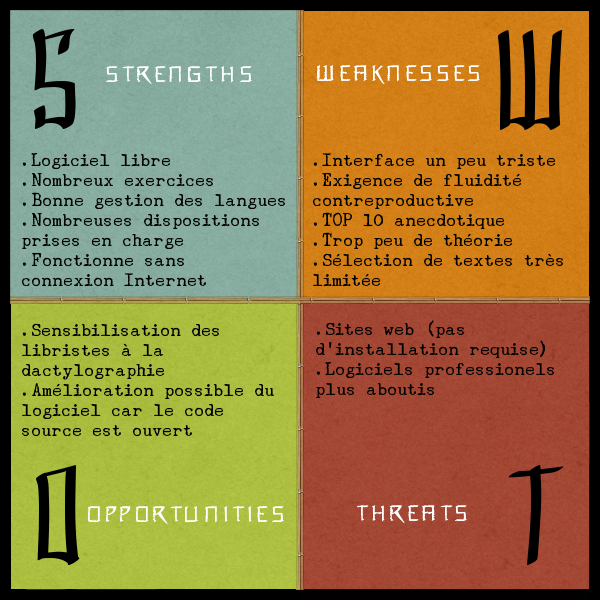
\includegraphics[scale=0.5]{swot-klavaro.png}
\end{center}
\caption{Matrice SWOT - Klavaro}
\end{figure}

\newpage

\subsubsection{10FastFingers}

10FastFingers est un site web multilingue qui s'appuie majoritairement sur la vitesse de frappe. Sur ce site, l'épreuve reine est un test de dactylographie où l'utilisateur doit saisir le plus vite possible une série de mots générée aléatoirement. Dans le test classique, cette série est générée à partir des 200 mots les plus courants de la langue choisie. Dans le test avancé, cette série est générée à partir des 1000 mots les plus courants de la langue choisie. Les résultats aux tests alimentent des classements par langue et on peut obtenir un suivi précis de nos performances sous forme de graphiques, à condition de créer un compte.

Un mode entraînement (\og~Top 1000~\fg) est également disponible. Ce dernier permet à l'utilisateur de s'exercer sur des séries contenant les mots les plus courants de la langue choisie. Aucun score obtenu ici n'est public. L'idée est simplement de se préparer tranquillement aux tests de dactylographie.

Un mode compétition permet aussi aux utilisateurs de s'affronter en dehors des classements traditionnels. Le principe est simple~: un membre crée une compétition (privée ou publique) dans une langue spécifique. Cette compétition dure nécessairement 24 h et la série de mots (générée aléatoirement) est toujours la même. À l'issue des 24 h, le vainqueur est celui qui a fait le meilleur score sur la série de mots. Le nombre d'essais n'est pas limité.

Récemment, la possibilité de pratiquer la frappe sur des textes personnalisés a aussi été ajoutée. Cette fonctionnalité reste cependant en retrait. Une application Android est aussi proposée pour travailler la vitesse de frappe à deux pouces sur écran tactile. Mais là-encore, cette fonctionnalité reste quelque peu en retrait.

Par ailleurs, 10FastFingers est un site ludique car des récompenses symboliques sont attribuées aux utilisateurs qui atteignent certains objectifs (dépassement d'une certaine vitesse, d'un certain nombre de tests, d'un certain nombre de participations et de victoires aux compétitions, etc.). De même, les derniers tests effectués par les utilisateurs alimentent un petit fil d'actualités, et il est possible de partager un score sur les réseaux sociaux. Un forum phpBB indépendant est aussi mis à disposition des internautes, bien qu'il soit assez anecdotique.

\begin{figure}
\begin{center}
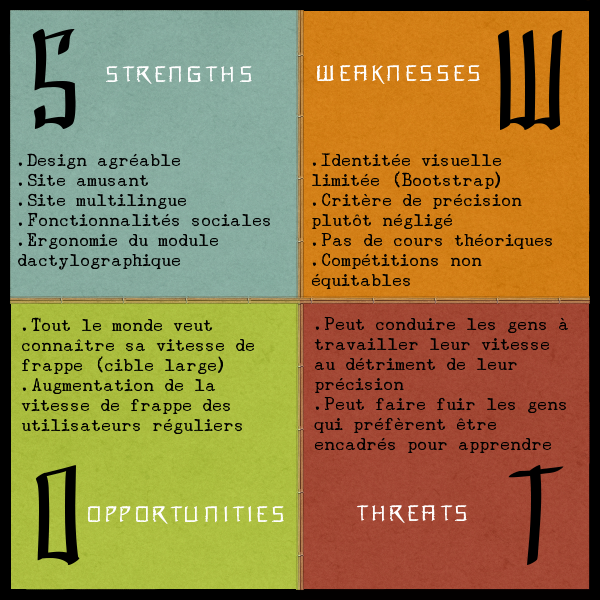
\includegraphics[scale=0.5]{swot-10ff.png}
\end{center}
\caption{Matrice SWOT - 10FastFingers}
\end{figure}

\newpage

\subsubsection{Keyhero}

Keyhero est un site web multilingue misant sur la dimension collaborative, et notamment sur le crowdsourcing ou UGC (User-Generated Content). Comme la plupart des sites portant sur la dactylographie, Keyhero propose des conseils, des tutoriels, des exercices pour s'entraîner... Jusque-là, rien de bien original. Mais le cœur de Keyhero, c'est la saisie de textes ajoutés par les utilisateurs. En fait, le contenu des tests dactylographiques est ajouté par les utilisateurs eux-mêmes, et un système de vote permet de valoriser ou de dévaloriser certains textes.

Ici, la vitesse et la précision sont d'égale importance. Un système précis de détection des erreurs a d'ailleurs été mis en place pour que l'utilisateur puisse bien comprendre les erreurs qu'il commet. Parmi les erreurs répertoriées, on retrouve~:

\begin{itemize}
 \item{Erreurs de casse}
 \item{Interversions de lettres}
 \item{Caractères doublés}
 \item{Divers}
\end{itemize}

Ce qui est intéressant dans la gestion des erreurs, c'est la pénalité qui est attribuée à l'utilisateur s'il ne les corrige pas. Sur Keyhero, contrairement à d'autres sites sur lesquels la saisie est bloquée en cas d'erreur, l'utilisateur est libre ou non de corriger ses fautes de frappe. S'il ne le fait pas, son score final est automatiquement revu à la baisse.

Sur Keyhero, des récompenses sont également attribuées aux utilisateurs qui atteignent certains objectifs en termes de vitesse, de précision, et d'ajout de citations (textes). Mais cette fonctionnalité est largement anecdotique ici car elle n'est pas suffisamment élaborée pour apporter cet aspect ludique qu'on peut retrouver sur d'autres sites.

Naturellement, tous les membres de Keyhero disposent d'une page de profil où chacun peut avoir un compte rendu des performances réalisées. Tout membre peut également poster un message sur le forum intégré au site web.

\begin{figure}
\begin{center}
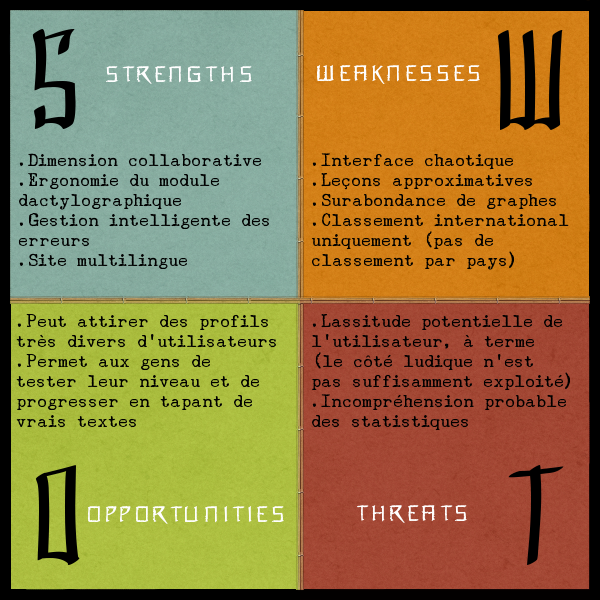
\includegraphics[scale=0.5]{swot-keyhero.png}
\end{center}
\caption{Matrice SWOT - Keyhero}
\end{figure}

\newpage

\subsubsection{Nitro Type}

Nitro Type est un site web à dimension internationale, restant malgré tout purement anglophone. L'interface est exclusivement en anglais, de même que les contenus à taper. Cependant, nous ne pouvions pas ne pas présenter ce site qui est clairement l'une des applications les plus abouties en matière de dactylographie. Aucun équivalent n'existe d'ailleurs en français.

Nitro Type est bien plus qu'un simple site web proposant de pratiquer la dactylographie au quotidien. C'est carrément un jeu à part entière avec un graphisme soigné, des défis à la pelle, des récompenses, des niveaux avec points d'expérience (XP), des compétitions, et bien d'autres choses...

Comme le suggère plus ou moins le nom du site, Nitro Type est un jeu de course faisant intervenir des véhicules en tout genre, mais plus particulièrement des voitures. L'utilisateur souhaitant profiter au maximum des fonctionnalités offertes doit se créer un compte (gratuitement). Il commence alors son aventure sans XP, sans argent, et avec une voiture bas de gamme. Ensuite, au fur et à mesure des courses et des victoires, le membre gagne de l'expérience, de l'argent, débloque des bonus. Il peut acheter de nouveaux véhicules pour frimer un peu ou les fameuses nitros qui permettent de sauter des mots lors d'une course. Car, oui, Nitro Type est avant tout un jeu de course dactylographique. L'épreuve au centre du jeu est un test classique, à la différence près que notre progression est matérialisée par l'avancée d'un véhicule en temps réel, tout comme celle des quatre autres concurrents qui partagent la course.

Sur Nitro Type, l'utilisateur a accès à de nombreuses fonctionnalités utiles et ludiques, comme un rapport statistique détaillé de ses performances et de son activité, ou encore le garage où il peut entreposer ses véhicules et en changer quand bon lui semble. Sur le site, il est possible d'ajouter des membres à sa liste d'amis, et même de rejoindre des équipes en fonction de certains critères. Ceci a bien sûr une incidence sur les classements où il est possible de s'illustrer individuellement ou collectivement en termes de vitesse et d'activité.

\begin{figure}
\begin{center}
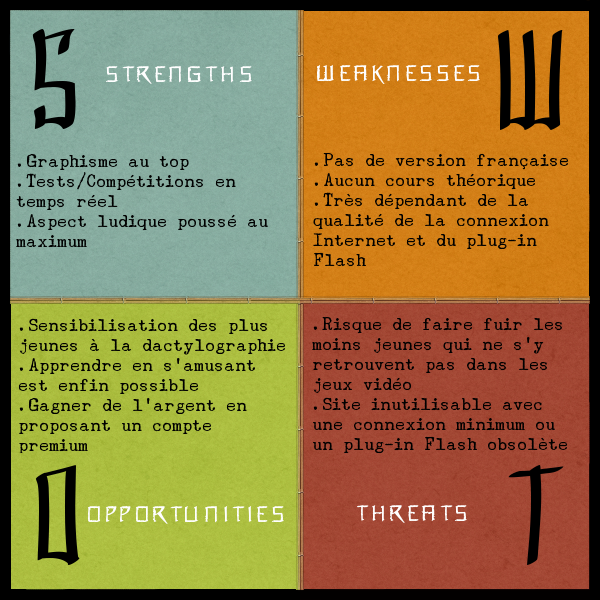
\includegraphics[scale=0.5]{swot-nitrotype.png}
\end{center}
\caption{Matrice SWOT - Nitro Type}
\end{figure}

\subsection{Apprentissage de la dactylographie pour programmeurs}

Dans cette partie nous allons voir les sites qui peuvent être considérés comme les leaders en matière de dactylographie pour programmeurs~: Typing.io et SwiftCODE.

\subsubsection{Typing.io}

Typing.io est un site qui permet à ses utilisateurs d'apprendre à mieux taper du code. Le site dispose d'un certain nombre de fonctionnalités intéressantes, notamment statistiques, qui ne ne sont malheureusement pas accessibles gratuitement. Il n'est pas non plus possible d'ajouter ses propres morceaux de code sans payer la modique somme de 9,99~\$ par mois...

Malgré tout, Typing.io met à disposition un certain nombre de leçons gratuites, ce qui est d'ailleurs suffisant pour ceux qui veulent juste se tester ou pratiquer la saisie de code, sans forcément avoir tout l'attirail analytique qui va avec. Ces leçons sont classées par langage informatique (JavaScript, Java, PHP, C++, etc.) et par projet (jQuery, Symfony, Webkit, etc.).

Une fois le projet sélectionné, l'utilisateur doit taper des morceaux de code qui en sont issus. De manière assez classique, le programme lui signale quand la saisie est correcte et quand elle est incorrecte. Pour des raisons de lisibilité, l'indentation du code est conservée et les tabulations ne sont pas à taper. À l'issue de la session, l'utilisateur reçoit un mini-rapport l'informant de ses performances.

\begin{figure}
\begin{center}
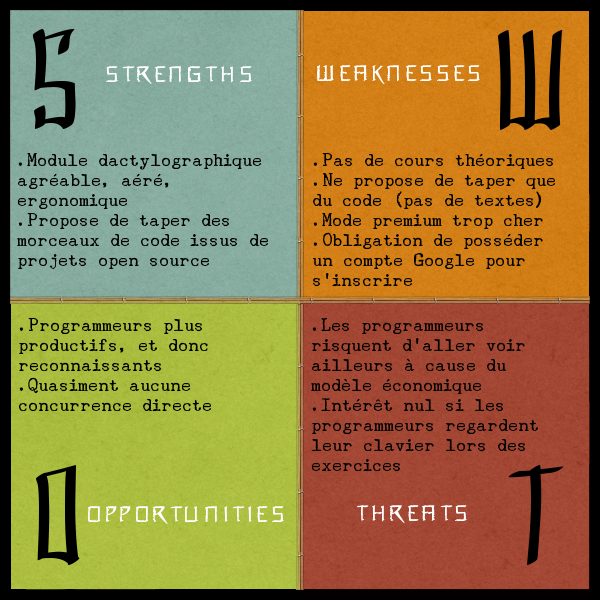
\includegraphics[scale=0.5]{swot-typingio.png}
\end{center}
\caption{Matrice SWOT - Typing.io}
\end{figure}

\subsubsection{SwiftCODE}

SwiftCODE se présente comme un jeu multijoueur de vitesse dactylographique pour programmeurs. En réalité, SwiftCODE dispose d'un mode solo et d'un mode multijoueur. Le mode solo permet de s'entraîner sur divers langages informatiques, du HTML au Java, en passant par TeX, Python et JavaScript. Le mode multijoueur, quant à lui, permet d'affronter en temps réel d'autres programmeurs sur la saisie d'un morceau de code dans le langage choisi. Lors de la saisie, le programme signale évidemment à l'utilisateur lorsqu'il tape correctement et lorsqu'il fait des fautes. À l'issue du test, un rapport assez classique est affiché, avec vitesse, précision, etc.

\begin{figure}
\begin{center}
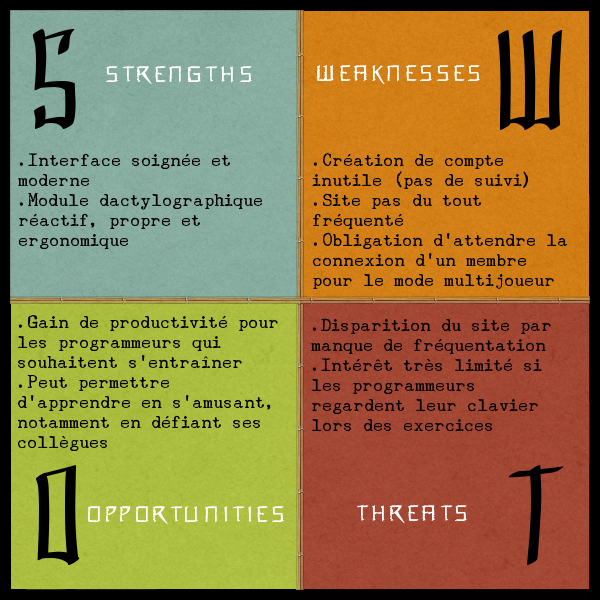
\includegraphics[scale=0.5]{swot-swiftcode.png}
\end{center}
\caption{Matrice SWOT - SwiftCODE}
\end{figure}

\newpage

% ==========================================================================
% ======================= II. Présentation du site =========================
% ==========================================================================

\part{Présentation du site}

Nous avons pu détailler le contexte du projet, mais il nous incombe maintenant de présenter de manière exhaustive ce que propose Dojoctylo et comment il le propose. Nous allons donc ici aborder la charte graphique, le modèle de navigation, ainsi que les fonctionnalités proposées à l'internaute.

\section{Le projet en quelques mots}

Dojoctylo a été pensé pour être un site web amusant et moderne où tout le monde peut apprendre la dactylographie par le biais de cours théoriques et d'exercices pratiques. Le site se concentre sur les dispositions francophones (AZERTY, BÉPO, Dvorak-fr), trop souvent passées à la trappe ou mal expliquées. Comme dans un jeu, les membres se voient attribuer des récompenses en fonction de leurs performances et de leur activité. Dojoctylo est définitivement le berceau des ninjas du clavier~!

\section{Charte graphique}

Pour se démarquer de la concurrence, y compris internationale, une grande attention a été portée au graphisme. C'est en effet le graphisme qui donne toute sa personnalité à un site web, et en l'occurrence, la plupart des sites qui traitent de la dactylographie sont assez ternes. Ils valideraient presque l'idée selon laquelle la dactylographie est une pratique has-been pour secrétaires à la retraite...

Dojoctylo se démarque justement grâce à une charte graphique colorée et chaleureuse qui a pour objectif de donner envie aux gens de se mettre à la dactylographie. Dojoctylo a pour ambition de montrer que la dactylographie n'est pas qu'une pratique austère~; on peut donc tout à fait apprendre quelque chose d'utile en s'amusant. Le choix de la thématique n'est d'ailleurs pas anodin. Dans l'imaginaire collectif, les ninjas, c'est avant tout de l'action, des arts martiaux, et des combats épiques. Mais c'est aussi un entraînement rigoureux avec un maître qui dispose de la sagesse. Pour des raisons de cohérence avec le thème, le graphisme s'inspire donc des couleurs, des textures, et des formes que l'on retrouve communément dans un dojo~; cet espace d'entraînement où les ninjas se dépassent et progressent au combat. Le nom du site lui-même, \og~Dojoctylo~\fg, est une contraction entre \og~dojo~\fg{} et \og~dactylo~\fg~; comme vous l'aviez probablement déjà deviné. Maître Taipingu, le personnage emblématique du site, s'appelle d'ailleurs ainsi car \og~taipingu~\fg{} signifie \og~dactylographie~\fg{} en japonais.

\begin{figure}[!h]
\begin{center}
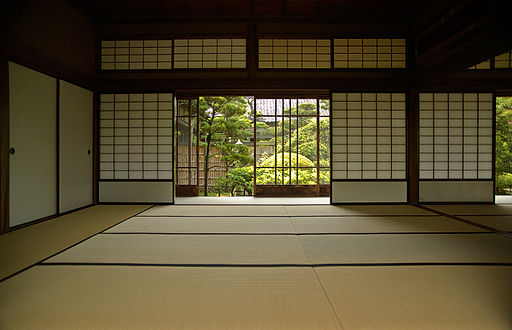
\includegraphics[width=\textwidth]{dojo.jpg}
\end{center}
\caption{L'architecture japonaise dans toute sa splendeur}
\end{figure}

Au niveau des couleurs, on retrouve bien sûr du brun et du beige pour rappeler la couleur du bois et des tatamis. On retrouve aussi du noir et du rouge pour cultiver une ambiance ninja.

Sur le plan des textures, on constate qu'il y a des quadrillages et des morceaux de bois qui évoquent notamment le shôji, cette paroi en papier de riz et bois si caractéristique de l'architecture japonaise. On retrouve aussi le bambou qui, pour nous occidentaux, a ce petit goût d'Asie.

Concernant les formes, l'internaute ne sera pas surpris de voir beaucoup de rectangles, comme dans l'architecture japonaise. La navigation très rectangulaire a d'ailleurs été inspirée des jeux de combat, lorsque le joueur doit choisir un mode ou un personnage.

Enfin, il est important de noter que l'intégralité des images utilisées sur Dojoctylo relèvent du domaine public ou disposent d'une licence Creative Commons qui permet une libre exploitation. Se reporter aux mentions légales du site pour de plus amples informations.

\section{Modèle de navigation}

La navigation du site a été conçue de telle sorte que l'utilisateur puisse accéder à n'importe quel contenu en trois clics maximum. En d'autres termes, la profondeur maximale est de trois sous-niveaux.

La navigation principale est constituée de trois liens qui amènent chacun vers une section fondamentale de Dojoctylo. En cliquant sur l'un de ces liens, l'utilisateur est amené sur une page où il peut choisir son mode d'apprentissage, de pratique, ou de compétition, à la manière d'un jeu de combat.

La page d'accueil, elle aussi, contient des liens vers les pages principales de Dojoctylo, ainsi que vers la page de récompenses et de connexion pour inciter l'internaute à s'inscrire.

Dans le footer, on retrouve quelques liens vers les pages secondaires, en l'occurrence~: les mentions légales, une FAQ, un lien de contact, un plan du site, et un classement des membres en fonction de leurs performances et de leur activité sur Dojoctylo.

\section{Fonctionnalités}

Dojoctylo a pour ambition de devenir une sorte de hub de la dactylographie, et en cela, il se doit de concentrer un grand nombre de fonctionnalités. Pour mettre en avant chacune d'elle, nous allons reprendre en partie le modèle de navigation évoqué plus haut. Le lecteur pourra ainsi comprendre avec précision ce que propose Dojoctylo, sans même avoir visité le site.

\subsection{Apprendre}

Pour apprendre la dactylographie, il faut commencer par suivre des leçons théoriques. L'utilisateur de Dojoctylo pourra bien sûr faire des tests et des exercices pratiques sans maîtriser les rudiments de la discipline, mais ce n'est pas le but de la manœuvre. Sur Dojoctylo, il convient donc de proposer des conseils ainsi que des tutoriels pour bien taper au clavier. L'ergonomie étant indispensable pour éviter les problèmes de santé, il convient aussi d'en parler.

\subsubsection{Conseils}

Cette section est relativement simple puisqu'elle propose, un peu sous la forme de commandements, ce qu'il faut faire et ne pas faire pour devenir un bon dactylographe. L'utilisateur est ensuite libre de suivre ces conseils avisés ou non, mais en tout cas c'est un premier pas vers l'apprentissage. Comme souvent dans la vie, mieux vaut prendre les bonnes habitudes tout de suite car gommer de mauvaises habitudes n'a rien d'évident.

\subsubsection{Tutoriels}

Pour celles et ceux qui souhaitent aller plus loin que de simples conseils, Dojoctylo propose plusieurs tutoriels répartis par niveaux et dispositions. Ainsi l'utilisateur débutant peut commencer par lire un tutoriel qui lui apprend à découvrir son clavier, pendant que l'utilisateur expérimenté peut perfectionner sa connaissance du clavier avec la saisie de caractères typographiques rares.

À l'heure actuelle, Dojoctylo ne contient que trois tutoriels, l'un étant facile, l'autre intermédiaire, et le dernier difficile. La disposition traitée n'est pour l'instant que l'AZERTY, mais le BÉPO et le Dvorak-fr devraient faire leur apparition quand l'auteur de ces lignes aura eu le temps de les tester...

\subsubsection{Ergonomie}

Cette page a pour but de proposer, de manière totalement objective (entendez par là qu'il n'y a pas de contenu sponsorisé), des modèles de clavier qui sortent un peu de l'ordinaire et qui ont pour vocation d'être ergonomiques. Il n'y a pour l'instant pas de texte qui décrit avec précision les avantages et les inconvénients des différents modèles. Ceci viendra certainement avec le temps pour améliorer le référencement. En tout cas, l'utilisateur peut d'ores et déjà avoir une idée de ce qui se fait en dehors des sentiers battus en matière de claviers, donc libre à lui ensuite d'expérimenter par ses propres moyens.

\subsection{Pratiquer}

La théorie, c'est bien. Mais comme disait Einstein~: \textit{\og~La théorie, c'est quand on sait tout et que rien ne fonctionne. La pratique, c'est quand tout fonctionne et que personne ne sait pourquoi. Ici, nous avons réuni théorie et pratique~: Rien ne fonctionne... et personne ne sait pourquoi !~\fg}

Autrement dit, il y a peu de chances que vous soyez un bon dactylographe si vous vous limitez uniquement à la théorie ou uniquement à la pratique. En plus de lire soigneusement ce qui se passe dans la section \og~Apprendre~\fg, tout utilisateur sérieux devra passer beaucoup de temps dans la section \og~Pratiquer~\fg~!

Dans cette section, on retrouve un grand nombre d'exercices divers et variés, et pour chacun d'entre eux, trois niveaux de difficulté sont proposés~: facile, moyen, et difficile.

\subsubsection{Bases}

Ce mode de pratique a été conçu pour permettre aux utilisateurs de découvrir leur clavier. Ici, l'utilisateur se concentre uniquement sur les caractères à taper. Il n'y a donc pas de phrases, ni même de mots. Le tout n'a d'ailleurs aucun sens. Le but est vraiment de travailler la mémoire musculaire à l'échelle du caractère.

En \textbf{mode facile}, il s'agit globalement de taper des séries contenant deux lettres de la même rangée, dont l'une est à gauche du clavier et l'autre à droite. Ceci est une première approche pour bien dissocier ce qui doit être tapé par la main gauche et ce qui doit être tapé par la main droite.

En \textbf{mode moyen}, l'utilisateur doit saisir des séries contenant plusieurs lettres adjacentes. L'idée est ici de travailler la dextérité des doigts de la main.

En \textbf{mode difficile}, les choses se corsent réellement puisque l'ensemble du clavier peut être sollicité. Les lettres ne sont plus forcément sur la même rangée ni même consécutives. Par ailleurs, les majuscules, les caractères accentués et la ponctuation usuelle répondent à l'appel, ce qui sous-entend l'utilisation massive des touches modificatrices (en particulier \og~Shift~\fg{} et \og~Caps Lock~\fg).

\subsubsection{Digrammes}

\textit{\og~En linguistique, un digramme est un assemblage de deux signes (généralement deux lettres dans un alphabet), diacritiques non comptés, formant un unique graphème, et représentant ainsi un unique phonème.~\fg} (Source~: Wikipédia)

L'idée derrière ce mode de pratique est de s'exercer sur des digrammes courants, en particulier sur les assemblages de deux lettres qui reviennent le plus souvent dans la langue française.

En \textbf{mode facile}, l'utilisateur doit taper des séries de digrammes doublés, c'est-à-dire qui contiennent deux fois la même lettre.

En \textbf{mode moyen}, il s'agit de taper des séries de digrammes simples, non doublés. Autrement dit, les deux lettres du digramme sont différentes, mais il n'y a aucun accent dans l'exercice.

En \textbf{mode difficile}, les séries contiennent des accents et les deux lettres de chaque digramme sont uniques.

\subsubsection{Trigrammes}

\textit{\og~En linguistique, un trigramme est une association de trois signes, diacritiques éventuels non comptés, formant un graphème et représentant ainsi un phonème unique.~\fg} (Source~: Wikipédia)

Cet exercice est très similaire au précédent, à la différence près que l'utilisateur doit ici taper des séries de trois lettres consécutives qui reviennent le plus souvent dans la langue française.

En \textbf{mode facile}, le trigramme à taper contient deux lettres identiques.

En \textbf{mode moyen}, le trigramme à taper contient trois lettres simples et uniques.

En \textbf{mode difficile}, le trigramme à taper contient trois lettres uniques, avec accents, cédilles, etc.

\subsubsection{Mots}

Si l'utilisateur suit assidûment le parcours, dans l'ordre, c'est à partir d'ici que les choses deviennent réellement intéressantes pour lui. Contrairement à ce que l'on pourrait penser de prime abord, s'exercer sur des caractères, des digrammes et des trigrammes n'a rien d'inutile. En effet, un mot est composé de caractères, par extension de digrammes, par extension de trigrammes. Un dactylographe particulièrement habile avec les digrammes et trigrammes usuels sera plus efficace qu'un dactylographe qui raisonne uniquement à l'échelle du caractère.

Toujours est-il qu'ici, l'objectif est de saisir des séries de mots différents.

En \textbf{mode facile}, l'utilisateur doit saisir des mots très simples qui ne posent aucune difficulté. Ce sont en général des mots courts, sans accents, et qui ne nécessitent aucun recours aux touches modificatrices.

En \textbf{mode moyen}, les mots à saisir sont un peu plus complexes, mais rien d'insurmontable. Les mots appartiennent généralement à un langage courant et font partie du vocabulaire universel.

En \textbf{mode difficile}, les mots sont globalement longs et représentent un vrai défi, aussi bien pour les lire que pour les taper... Ce sont des mots appartenant à un langage soutenu, technique, scientifique, ou tout simplement spécialisé.

\subsubsection{Phrases}

Ici, l'utilisateur peut naturellement mettre en pratique ce qu'il a appris en tapant des mots ; une phrase étant grosso modo un assemblage de mots...

En \textbf{mode facile}, l'utilisateur doit saisir des phrases simples, aussi bien sur le plan du sens que sur celui de la frappe au clavier.

En \textbf{mode moyen}, rien de révolutionnaire, si ce n'est que la difficulté monte d'un cran.

En \textbf{mode difficile}, l'utilisateur est confronté à des phrases alambiquées qui utilisent un maximum de caractères différents et spéciaux du clavier. Les pangrammes, notamment avec les lettres accentuées, sont ici récurrents.

\textit{\og~Un pangramme [...] est une phrase comportant toutes les lettres de l'alphabet.~\fg} (Source~: Wikipédia)

\subsubsection{Nombres}

Les nombres ont une existence à part entière dans le petit monde de la dactylographie. Leur pratique est un peu particulière, notamment en fonction du matériel et du système d'exploitation dont on dispose. Ainsi, par exemple, un utilisateur sous Linux sans pavé numérique n'aura pas du tout les mêmes habitudes à prendre qu'un utilisateur sous Windows avec un pavé numérique.

Comme on peut s'en douter, le but de l'exercice est donc de taper des nombres. Là encore, la pratique est répartie en trois modes de difficulté.

En \textbf{mode facile}, il s'agit de taper des séries de deux chiffres, en alternant entre un chiffre à gauche du clavier et un autre à droite. On suppose ici que l'utilisateur n'a pas de pavé numérique.

En \textbf{mode moyen}, l'utilisateur doit taper des séries de plusieurs chiffres consécutifs pour travailler la dextérité des doigts de la main. Là encore, on suppose que l'utilisateur n'a pas de pavé numérique.

En \textbf{mode difficile}, l'utilisateur doit taper des séries contenant tous les chiffres, plus tous les opérateurs arithmétiques de base. Sans pavé numérique, cette épreuve est un cauchemar...

\subsubsection{Textes}

Sans aucun doute l'épreuve reine en dactylographie~: la saisie de textes. Dans le cas présent, l'utilisateur est amené à taper de petits morceaux de textes~; il va de soi qu'il n'est pas raisonnable de le faire taper des manuscrits de plusieurs milliers de pages...

En \textbf{mode facile}, l'utilisateur est confronté à des textes simples à comprendre et à taper. Les touches modificatrices sont rarement utilisées, de même que les accents ou les caractères spéciaux.

En \textbf{mode moyen}, les textes sont un peu plus compliqués, aussi bien sur le fond que sur la forme. Cependant, la difficulté reste très raisonnable.

En \textbf{mode difficile}, les ennuis commencent avec des textes alambiqués. Ce sont globalement des textes qui requièrent un usage intensif des touches modificatrices, des nombres, et autres joyeusetés du même genre. Généralement en langage soutenu, technique, scientifique, ou du moins spécialisé, ces textes ont de quoi donner du fil à retordre.

\subsubsection{Code}

Créé avant tout pour les codeurs, cet exercice est néanmoins ouvert à tous. Il permet de travailler sa frappe avec des morceaux de code plus ou moins difficiles.

En \textbf{mode facile}, l'utilisateur doit taper du code assez simple. Par \og~simple~\fg, on entend par exemple~: HTML, CSS, XML, JSON, etc. Ces langages sont facilement lisibles et compréhensibles, même par des gens qui ne sont pas forcément des programmeurs chevronnés. Ces langages ont aussi l'avantage de ne pas être très difficiles à taper.

En \textbf{mode normal}, l'utilisateur doit taper des morceaux de programmes qui n'ont rien de simple. Ici, on peut retrouver n'importe quel langage de programmation, tel que JavaScript, PHP, Java, Python, C, etc.

En \textbf{mode difficile}, l'utilisateur risque de transpirer car il s'agit en général de taper des fichiers de configuration particulièrement complexes, avec énormément de caractères spéciaux, d'expressions régulières, etc.

\subsubsection{Sur-mesure}

L'utilisateur a déjà de quoi faire avec l'ensemble des modes de pratique proposés par Dojoctylo. Mais si l'utilisateur estime que cela n'est pas suffisant, il a aussi la possibilité de construire ses propres exercices en important du contenu personnalisé. Bien sûr, pour rester cohérent avec ce qui est déjà proposé par ailleurs, l'utilisateur peut choisir de répartir ses exercices personnalisés en plusieurs modes de difficulté~: facile, moyen, et difficile.

\subsection{Affronter}

Pratiquer tout seul, c'est bien. Mais c'est aussi intéressant de pouvoir affronter les autres pour montrer de quel bois on se chauffe~! À ce titre, Dojoctylo propose plusieurs compétitions~: un mode solo, des compétitions privées, et enfin des compétitions publiques.

\subsubsection{Test (mode solo)}

Ici l'utilisateur est seul face au chronomètre. Il dispose d'une minute pour taper le texte qui s'affiche dans le module dactylographique. À l'issue du chronomètre, l'utilisateur reçoit un score composé d'une vitesse en mots par minute (MPM) et d'une précision en pourcentage (\%).

\subsubsection{Défi (compétition privée)}

Une compétition privée est une compétition entre amis, autrement dit entre membres connectés sur Dojoctylo.

Ce mode n'a pas encore été développé. Se reporter à la dernière section du rapport, sur les perspectives d'évolution, pour plus d'informations.

\subsubsection{Tournoi (compétition publique)}

Une compétition publique est une compétition ouverte à tous les membres de Dojoctylo.

Ce mode n'a pas encore été développé. Se reporter à la dernière section du rapport, sur les perspectives d'évolution, pour plus d'informations.

\subsection{Divers}

En plus des fonctionnalités explicitées précédemment, il convient maintenant de citer l'espace membre ainsi que le classement.

\subsubsection{Espace membre}

L'espace membre de Dojoctylo permet aux utilisateurs de sauvegarder leurs scores, de recevoir des récompenses pour leur investissement personnel, et tout simplement de disposer d'une page de profil. Des fonctionnalités sociales sont à prévoir à l'avenir. Se reporter encore une fois à la dernière section du rapport, sur les perspectives d'évolution, pour plus d'informations.

L'espace membre de Dojoctylo est relativement simple. Le pivot de cet espace est la page de profil, sur laquelle le membre peut voir son pseudo, avec éventuellement un avatar et une description riche. Sur cette page de profil, on trouve aussi un compte rendu d'activité, un graphe illustrant les dernières performances, ainsi que la liste complète des récompenses obtenues.

Naturellement, le membre est libre de modifier ses informations de profil à tout moment, sauf ses statistiques d'activité, ses scores et récompenses pour des raisons évidentes.

\subsubsection{Classement}

Le but d'un classement est avant tout d'insuffler une dimension ludique à l'apprentissage. Pour celles et ceux qui ont l'esprit de compétition, le classement va être une source de motivation et va donc encourager le dépassement de soi.

Le classement sur Dojoctylo prend en compte les résultats au test de dactylographie (mode solo, contre le chronomètre). Il est alors possible de voir les meilleures performances du jour, de la semaine, du mois, de l'année... Un classement global est également disponible.

Il va de soi que les scores des utilisateurs non connectés n'apparaissent pas dans ce classement. Ces scores ne sont d'ailleurs pas enregistrés.

\newpage

% ==========================================================================
% ====================== III. Réalisation technique ========================
% ==========================================================================

\part{Réalisation technique}

Dojoctylo a été conçu ex nihilo, sans CMS ni solution clé en main. Nous développerons tout l'aspect technique dans cette partie, en commençant par le front-end et en terminant par le back-end. Mais avant cela, voici déjà un aperçu de l'architecture globale de l'application avec un bref descriptif du rôle de chaque dossier :

\begin{figure}[!h]
\begin{center}
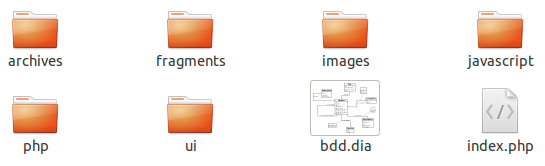
\includegraphics[scale=0.5]{architecture-globale.png}
\end{center}
\caption{Architecture globale de Dojoctylo}
\end{figure}

\begin{itemize}
 \item{\textbf{archives :} Contient les anciennes versions des différentes pages du site. Sert à faire du versioning basique, sans Git ou SVN.}
 \item{\textbf{fragments :} Contient tous les fragments d'informations et de scripts qui sont appelés lors de la construction dynamique des pages en PHP.}
 \item{\textbf{images :} Contient toutes les images de contenu et celles de la charte graphique.}
 \item{\textbf{javascript :} Contient toutes les librairies et tous les scripts JavaScript utilisés. Le module dactylographique se trouve ici.}
 \item{\textbf{php :} Contient toute la partie back-end, et donc toutes les classes et librairies en PHP.}
 \item{\textbf{ui :} Contient les feuilles de style CSS, les polices, et les templates.}
\end{itemize}

Le schéma de base de données et le contrôleur seront abordés plus tard, dans la partie back-end...

\newpage

\section{Front-end}

La partie front-end de Dojoctylo comprend l'intégration des pages et le développement du module dactylographique.

\subsection{Intégration}

Dojoctylo a été structuré en utilisant le balisage mis à disposition par HTML5, il a été mis en forme avec CSS3, puis certaines pages ont été dynamisées à l'aide de JavaScript (en particulier jQuery) pour apporter plus d'ergonomie.

\subsubsection{HTML (HyperText Markup Language)}

La structure globale du site est assez classique, dans le sens où l'on retrouve un header, une navigation principale, ainsi qu'un footer sur chacune des pages. Dans la mesure où l'intégration a été réalisée en HTML5, ce sont bien entendu les éléments \og~header~\fg, \og~nav~\fg, et \og~footer~\fg{} qui ont été utilisés.

En dehors de ces éléments statiques, chaque page du site contient une division (\og~div~\fg) ou section principale (élément \og~section~\fg{} en HTML5) identifiée par un attribut \og~id~\fg. Comme un schéma vaut mieux qu'un long discours, voici à quoi ressemble le squelette du site~:

\newpage

\begin{figure}[!h]
\begin{center}
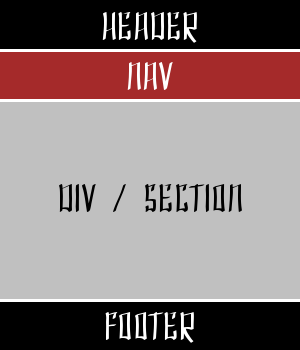
\includegraphics{structure.png}
\end{center}
\caption{Squelette HTML5 de Dojoctylo}
\end{figure}

\newpage

\subsubsection{CSS (Cascading Style Sheets)}

Dojoctylo dispose de trois feuilles de style conformes à la recommandation CSS3. Ces trois feuilles sont là pour permettre au site d'être responsive, afin qu'il puisse s'adapter à la taille de l'écran utilisé par l'internaute qui visite le site. Typiquement, on gère ici le cas du PC de bureau, de la tablette, et du smartphone.

Compte tenu du fait que Dojoctylo a été développé selon le paradigme \og~desktop-first~\fg{} (ce qui est logique puisqu'il s'agit d'un site de dactylographie...), la feuille de style qui gère l'affichage à partir de 1024 pixels de large est celle qui contient le plus de règles. Entre 600 pixels et 1023 pixels de large, la feuille intermédiaire surcharge quelques règles afin que l'affichage soit optimal. En deçà de 600 pixels de large, c'est la dernière feuille qui prend le relais.

Pour des raisons de lisibilité, et donc pour faciliter la maintenance du code, les règles CSS ont été réparties par groupes, en fonction de leur portée. Par exemple, une classe CSS qui concerne toutes les pages est classée dans la catégorie \og~global~\fg, alors qu'une règle spécifique à un élément d'une page est classée dans la catégorie portant le nom de la page. En outre, chaque sélecteur CSS spécifique reprend l'intégralité du chemin vers l'élément ciblé. Par exemple, si on veut cibler un élément \og~p~\fg{} à l'intérieur d'un article, qui est lui-même à l'intérieur d'une section, il est préférable d'utiliser le sélecteur \og~section article p~\fg{} que le sélecteur \og~p~\fg. Cette méthode de travail est certes un peu verbeuse, mais elle permet d'éviter les confusions et les problèmes de surcharge.

\subsubsection{JavaScript}

Sur Dojoctylo, toutes les pages contiennent du JavaScript. En dehors du module dactylographique que nous expliciterons peu après, JavaScript a principalement servi à faire des retouches ergonomiques, afin que l'expérience utilisateur soit optimale.

Pour tous les scripts JavaScript, c'est jQuery qui a été utilisé, notamment pour les facilités qu'apporte ce framework dans la manipulation du DOM (Document Object Model). En l'occurrence, jQuery a été utile pour faire un système de scroll semi-automatique et d'affichage dynamique sur la page des récompenses, des fenêtres pop-up personnalisées pour la modification du profil et la gestion des exercices sur-mesure, des tooltips pour guider l'utilisateur dans sa navigation, et bien entendu de la validation de formulaires côté client.

Pour le système de scroll semi-automatique et d'affichage dynamique, l'idée est juste de capter trois événements différents (\og~mouseover~\fg, \og~mouseout~\fg, \og~click~\fg) et de déclencher une action spécifique lorsque l'un d'eux est lancé. Ainsi~: 

\begin{itemize}
 \item{lorsque l'utilisateur survole une récompense, sa description s'affiche dans le titre}
 \item{lorsque l'utilisateur quitte la zone de survol de la récompense, sa description disparaît}
 \item{lorsque l'utilisateur clique sur une récompense, la fenêtre se positionne au bon endroit}
\end{itemize}

Quant aux fenêtres pop-up personnalisées, l'idée est simplement d'avoir quelque chose de mieux intégré que les fenêtres par défaut générées par JavaScript (cf. \og~alert~\fg, \og~confirm~\fg, etc.). Pour ce faire, le principe est d'insérer le bloc HTML à afficher directement dans le code source. Pour le transformer en pop-up, il suffit d'empêcher son affichage au chargement de la page avec la fonction \og~hide()~\fg{} de jQuery. Ensuite, quand l'utilisateur réalise une action (notamment un clic sur un bouton), on révèle le bloc HTML. Quand l'utilisateur a terminé (clic sur un bouton ou soumission d'un formulaire), on masque une nouvelle fois le bloc HTML ; le tout avec des transitions pour apporter de la fluidité aux différentes actions.

Pour ce qui est des tooltips, c'est notamment jQuery UI qui a été utilisé. L'avantage d'une tooltip est de proposer à l'internaute des \og~title~\fg{} bien mieux intégrés que l'effet de survol classique affiché par le navigateur. On gagne ainsi en interactivité, tout en allant plus loin dans la personnalisation du design.

Enfin, concernant la validation de formulaires, rien de bien révolutionnaire... Un plug-in jQuery aurait pu être utilisé, mais la validation est ici manuelle. Chaque champ de chaque formulaire est soigneusement vérifié pour s'assurer de l'intégrité des données. La plupart du temps, la validation s'assure au minimum que les champs ne soient pas vides, mais des expressions régulières sont aussi utilisées pour vérifier certains points bien précis~: composition du pseudo, longueur du mot de passe, validité de l'adresse e-mail, etc. Naturellement, un message d'erreur est affiché à l'internaute si quelque chose ne va pas dans ce qui a été saisi.

\textbf{N. B.} Pour offrir à l'internaute la possibilité d'ajouter une description enrichie à son profil, Dojoctylo intègre la version light de CKEditor qui est, il faut le dire, une application JavaScript !

\subsection{Module dactylographique}

Le module dactylographique est en quelque sorte le cœur du site puisque c'est lui qu'on retrouve dans tous les modes de pratique ainsi que dans les compétitions (du moins, dans le mode solo...). Ce dernier a été réalisé intégralement en JavaScript et communique avec le serveur en Ajax (Asynchronous JavaScript and XML), autrement dit en mode asynchrone. À noter que jQuery a encore une fois été utilisé dans le cadre du développement.

Ce module dactylographique contient en réalité deux scripts JavaScript~:

\begin{itemize}
 \item{Le premier se concentre sur la pratique (entraînement)}
 \item{Le deuxième se concentre sur le test dactylographique (compétition)}
\end{itemize}

Les deux scripts sont très similaires, mais pour éviter de se mélanger les pinceaux, il n'était probablement pas judicieux de n'en faire qu'un seul et même script. En effet~:

\begin{itemize}
 \item{En entraînement, il est important de faire la différence entre tous les modes de pratique. Ce n'est absolument pas le cas du test dactylographique où seuls les textes importent.\\}
 \item{En entraînement, il n'y a pas de compte à rebours. L'utilisateur peut donc taper des textes plus ou moins longs, et ce n'est qu'après avoir terminé la saisie que les scores sont affichés. Au cours du test, l'utilisateur ne peut plus rien taper au bout de 60 secondes. Ce point affecte donc le timer et les calculs finaux.\\}
 \item{À la fin d'un test, il est important d'envoyer les résultats à l'aide d'une requête POST asynchrone. Ceci est inutile dans le cadre de l'entraînement où les résultats n'ont pas vocation à être sauvegardés.\\}
 \item{Dans un simple exercice de pratique, l'utilisateur peut choisir son mode de difficulté. Lors d'un test dactylographique, il est parfaitement illogique de laisser l'utilisateur choisir son niveau de difficulté, en sachant que le classement n'en tient pas compte.}
\end{itemize}

Ceci étant dit, intéressons-nous maintenant au cœur du programme...

Le programme se décompose en trois grandes parties~:

\begin{enumerate}
 \item{Déclaration des variables globales (qui sont, de fait, utilisées un peu partout dans le script)}
 \item{Captation et gestion principale des événements}
 \item{Fonctions diverses}
\end{enumerate}

En programmation, il est souvent recommandé de ne pas utiliser trop de variables globales pour éviter les conflits de portée. Il est donc généralement préférable d'utiliser des variables locales dans ses scripts. Dans le cas présent, c'était assez naturel et bien plus pratique d'utiliser un certain nombre de variables globales. Parmi celles-ci, on trouve notamment l'id du caractère courant, le nombre de caractères tapés correctement, le nombre d'erreurs, le nombre de corrections, l'intervalle du timer, etc. La plupart des variables déclarées ici sont initialisées.

Après cette étape fondamentale, on entre véritablement au cœur du programme avec la fonction jQuery~: \$( document ).ready(function() {});

Dans cette fonction, on commence par gérer les spécificités de l'exercice. Si le module dactylographique est appelé dans un but d'entraînement, il faut d'abord déterminer quel est le mode qui a été sélectionné en récupérant cette valeur dans l'URL (Uniform Resource Locator). Tous les modes n'ayant pas le même nombre de contenus à l'heure actuelle, il est important de spécifier manuellement les effectifs pour chaque mode de pratique. On évite ainsi les déconvenues en Ajax lorsqu'on appelle un contenu qui n'existe pas... En effet, les contenus sont choisis aléatoirement, en utilisant cette fonction~:

\begin{lstlisting}
function selectionAleatoire() {

    // On choisit un nombre entre 0 et le nombre de contenus
    var nbAleatoire = Math.floor(Math.random() * nbContenus);
    
    // On constitue le chemin vers le fichier (variable globale)
    nomFichierSuivant = "javascript/dactylographie/contenus/" + mode + "/" + difficulte + "/" + nbAleatoire;
    
    // Si le fichier est identique, on relance
    while (nomFichierSuivant == nomFichierActuel) {
        nbAleatoire = Math.floor(Math.random() * nbContenus);
        nomFichierSuivant = "javascript/dactylographie/contenus/" + mode + "/" + difficulte + "/" + nbAleatoire;
    }
}
\end{lstlisting}


Ici, on voit bien qu'un problème se pose si l'on ne spécifie pas \og~nbContenus~\fg. N'ayant pas d'intervalle dans lequel générer un nombre aléatoire, le programme va générer n'importe quel nombre aléatoire qui ne correspond à aucun fichier (les fichiers sont nommés avec de simples numéros sur le serveur).

Si maintenant le module dactylographique est chargé pour effectuer un test, alors il faut masquer les options de sélection de difficulté qui n'ont pas lieu d'être.

Une fois que le contenu a été sélectionné par le programme, encore faut-il le charger... Dans le cas présent, c'est la fonction suivante qui réalise cette tâche~:

\begin{lstlisting}
function chargementContenu() {
    
    // Gestion visuelle du chargement pour l'utilisateur
    $( "#loader" ).show();
    $( "#source" ).hide();
    
    // Ajax
    $( "#a-taper" ).load(nomFichierSuivant, function() {
        
        nomFichierActuel = nomFichierSuivant;
        $( "#loader" ).hide();
        $( "#source" ).show();
        $( "#source" ).html( $( "#a-taper" ).find( "#infos" ).html() );
        
        // Formatage du texte
        var texteASaisir = $( "#contenu" ).text();
        texteASaisir = texteASaisir.replace(/'/g, "'");
        nbCaracteres = texteASaisir.length;
        
        // Injection de balises
        $( this ).html( "<span id=\"0\">" + texteASaisir.charAt(0) + "</span>");
        for (var i = 1; i < texteASaisir.length-1; i++) {
            if (texteASaisir.charAt(i) == "\n") {
                $( this ).append( "<br id=\"" + i + "\" />");
            } else {
                $( this ).append( "<span id=\"" + i + "\">" + texteASaisir.charAt(i) + "</span>");
            }
        }
        
        // Ajustements ergonomiques pour l'utilisateur
        clearStyle();
        clearScroll();
        clearPerformance();
        $( "#" + id ).addClass( "next" );
        $( "#zone-saisie" ).focus();
        $( "#zone-saisie" ).prop("readonly", false);
    
    });
}
\end{lstlisting}


Lorsqu'un contenu est en cours de chargement (c'est-à-dire lorsque le navigateur envoie une requête Ajax en l'attente d'une réponse), il faut que l'utilisateur soit au courant~; d'où l'utilisation d'un gif animé. Une fois que le contenu est chargé, on cache le gif, on extrait les informations du fragment HTML qui nous est renvoyé par le serveur. On en profite pour faire un peu de formatage à la volée et on construit la structure HTML du texte à taper, de sorte que chaque caractère soit facilement manipulable en JavaScript. Quelques ajustements ergonomiques sont finalement effectués pour améliorer l'expérience utilisateur.

Après chargement du contenu, l'utilisateur peut commencer à taper. À ce stade, ce sont les gestionnaires d'événements \og~input~\fg{} et \og~keydown~\fg{} qui vont prendre en charge la saisie de l'utilisateur. L'utilisateur va rencontrer trois styles de caractères au cours d'un exercice~:

\begin{itemize}
 \item{Gris~: le prochain caractère à taper}
 \item{Vert~: le caractère tapé est correct}
 \item{Rouge~: le caractère tapé est incorrect (à noter que la zone entière devient rouge dans ce cas) }
\end{itemize}

L'événement \og~input~\fg{} englobe ici la partie la plus importante du programme. Cet événement se déclenche en effet à chaque fois que le champ de saisie est modifié. C'est donc dans le gestionnaire de cet événement (qui est notamment une fonction anonyme) que l'on gère la plupart des touches saisies par l'utilisateur. À noter que la première modification du champ correspond à la première touche entrée par l'utilisateur. C'est précisément cette action qui déclenche le timer, si celui-ci n'est pas déjà actif...

La correction, quant à elle, n'est pas associée à l'événement \og~input~\fg{} mais à l'événement \og~keydown~\fg. En effet, \og~input~\fg{} ne permet pas de savoir si la touche de correction a été pressée ou non car la touche retour ne génère pas de caractère imprimable. Or il faut que l'on sache quand cette touche a été pressée pour pouvoir modifier en conséquence les différents compteurs du module (id du caractère courant, nombres d'erreurs, nombre de corrections, etc.).

Une fois que l'exercice ou test arrive à son terme, on calcule les résultats, on les insère dans le DOM, et on révèle le fragment HTML correspondant aux performances (ce dernier étant initialement caché). L'utilisateur reçoit alors sa vitesse et sa précision. Voici les formules mathématiques utilisées pour le calcul du score~:

\textbf{Entraînement :}

\begin{lstlisting}
 vitesse = Math.round(nbSaisiesOk / (5 * (secondes / 60)));
 precision = Math.round((nbSaisiesOk / (id + nbCorrections)) * 100);
\end{lstlisting}


\textbf{Test :}

\begin{lstlisting}
vitesse = Math.round(nbSaisiesOk / 5);
precision = Math.round((nbSaisiesOk / (id + nbCorrections)) * 100);
\end{lstlisting}

Enfin, le programme doit aussi gérer la modification du mode de difficulté par l'utilisateur, notamment dans le cas des exercices pratiques. Pour cela, il suffit simplement de capter le clic sur les différentes boutons mis à disposition de l'utilisateur et de rediriger ce dernier vers une nouvelle page contenant le mode de difficulté souhaité dans l'URL. Par défaut, les exercices sont en mode facile.

\section{Back-end}

Bien qu'elle ne soit pas visible, cette partie du développement représente un travail conséquent que nous allons ici présenter. Nous commencerons par une présentation de la base de données, puis nous parlerons du code produit en PHP orienté objet.

\subsection{Base de données}

N'étant pas une usine à gaz, Dojoctylo n'a que très peu d'informations à stocker en base de données. Le SGBD (Système de Gestion de Base de Données) utilisé dans le cadre du projet est MySQL. Le paradigme de conception est donc relationnel, et voici le schéma de référence en UML (Unified Modeling Language)~:

\begin{figure}[!h]
\begin{center}
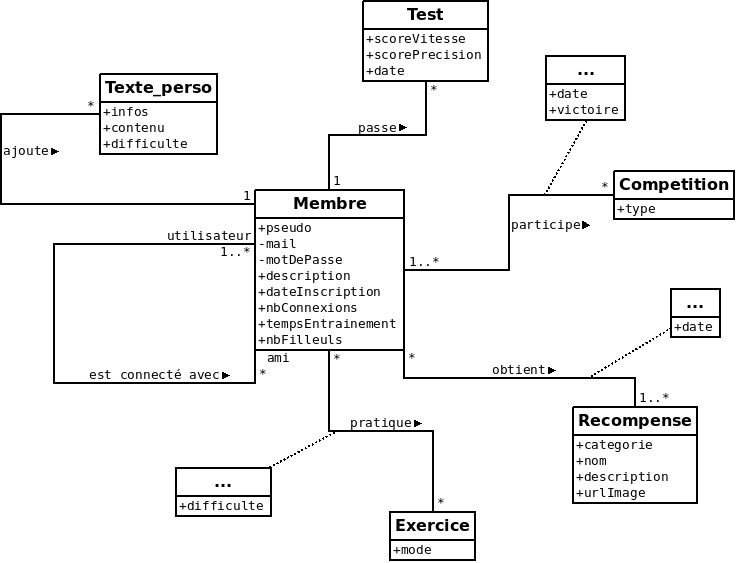
\includegraphics[scale=0.5]{bdd.png}
\end{center}
\caption{Schéma UML de la base de données}
\end{figure}

Ce schéma parle de lui-même... Compte tenu du fait que la base de données n'est utile que pour l'espace membre, il n'est pas surprenant de trouver une classe \og~Membre~\fg{} au cœur du schéma conceptuel.

Une fois implémenté physiquement via phpMyAdmin, ce schéma nous donne dix tables. En effet, chaque classe principale et chaque classe d'association (résultant d'une cardinalité maximale de type *-* pour une association) se transforme en table dans MySQL. Les associations avec cardinalité maximale de type 1-* ne donnent lieu qu'à une migration de clé primaire de la classe qui possède la plus petite cardinalité maximale vers celle qui possède la plus grande cardinalité maximale.

À noter la présence d'une relation récursive entre la classe \og~Membre~\fg{} et elle-même. Ici des rôles (utilisateur \& ami) sont précisés pour expliquer l'intérêt de cette relation~: un utilisateur est connecté avec aucun ou plusieurs amis, et un ami est connecté avec au moins un utilisateur. Bien sûr, un utilisateur et son ami sont tous les deux des membres. Pour matérialiser cela dans la base de données, il convenait de créer une table des amitiés contenant les identifiants des membres et ceux des relations de chacun.

À noter aussi que, puisqu'il s'agit d'un schéma UML, les clés primaires n'ont pas été mises en avant, bien qu'elles apparaissent distinctement. Les migrations et \og~fusions~\fg{} de clés primaires en clés étrangères n'apparaissent pas non plus pour ne pas embrouiller l'abstraction du modèle.

\subsection{Programmation orientée objet (POO)}

La partie immergée de Dojoctylo a été écrite en PHP. Elle s'articule autour d'une architecture sous forme de classes, en vertu du paradigme qu'est la programmation orientée objet. Ici nous allons donc tout naturellement présenter l'architecture mise en place. Nous profiterons également de cette partie pour évoquer les diverses mesures qui ont été prises en matière de sécurité informatique. Nous présenterons aussi l'API utilisée pour la gestion des photos de profil~: Gravatar.

\subsubsection{Architecture}

Le back-end de Dojoctylo s'appuie sur une architecture MVC (Modèle-Vue-Contrôleur). L'application dispose en effet d'un fichier principal, \og~index.php~\fg, qui joue le rôle de contrôleur. C'est dans ce fichier que l'ensemble des actions du site sont gérées, et donc c'est naturellement ici que le lien entre le modèle (base de données) et la vue (HTML) est établi. Le contrôleur a une visibilité publique, et c'est lui que l'utilisateur interroge lorsqu'il navigue sur le site.

Pour des raisons de clarté, les classes de Dojoctylo sont regroupées par packages, et donc par namespaces. Chaque package joue un rôle bien précis et contient, dans le cas le plus typique :

\begin{itemize}
 \item{Une classe qui construit une entité logique (e.g. classe \og~Membre~\fg)}
 \item{Une classe qui contient toutes les requêtes CRUD (Create, Read, Update, Delete) vers la base de données}
 \item{Une classe qui contient toutes les opérations afférentes à l'affichage (chargement de templates, construction de structures HTML, etc.)}
\end{itemize}

Le design pattern \og~Front Controller~\fg{} ou \og~contrôleur frontal~\fg{} n'ayant pas été implémenté, il n'y a pas encore de contrôleur spécifique à chaque package. Ceci devrait arriver à plus ou moins long terme afin de créer des modules autonomes.

Voici à quoi ressemble le c\oe ur de l'architecture back-end de Dojoctylo à l'heure actuelle :

\begin{figure}[!h]
\begin{center}
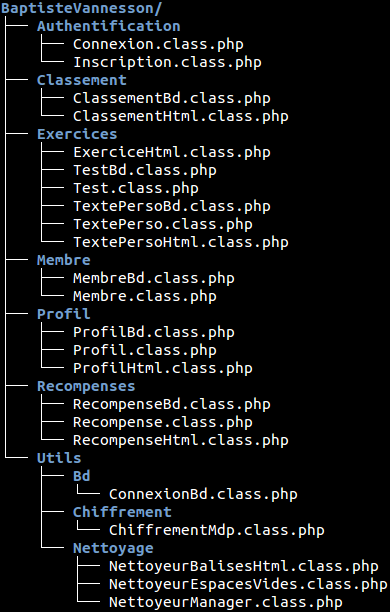
\includegraphics[scale=0.5]{architecture-backend.png}
\end{center}
\caption{C\oe ur de l'architecture back-end de Dojoctylo}
\end{figure}

Pour faciliter l'utilisation des namespaces, tous les packages sont eux-mêmes rassemblés dans un même dossier avec un nom de \og~vendor~\fg{} (ici \og~BaptisteVannesson~\fg).

En UML, ça donne ça :

\begin{figure}[!h]
\begin{center}
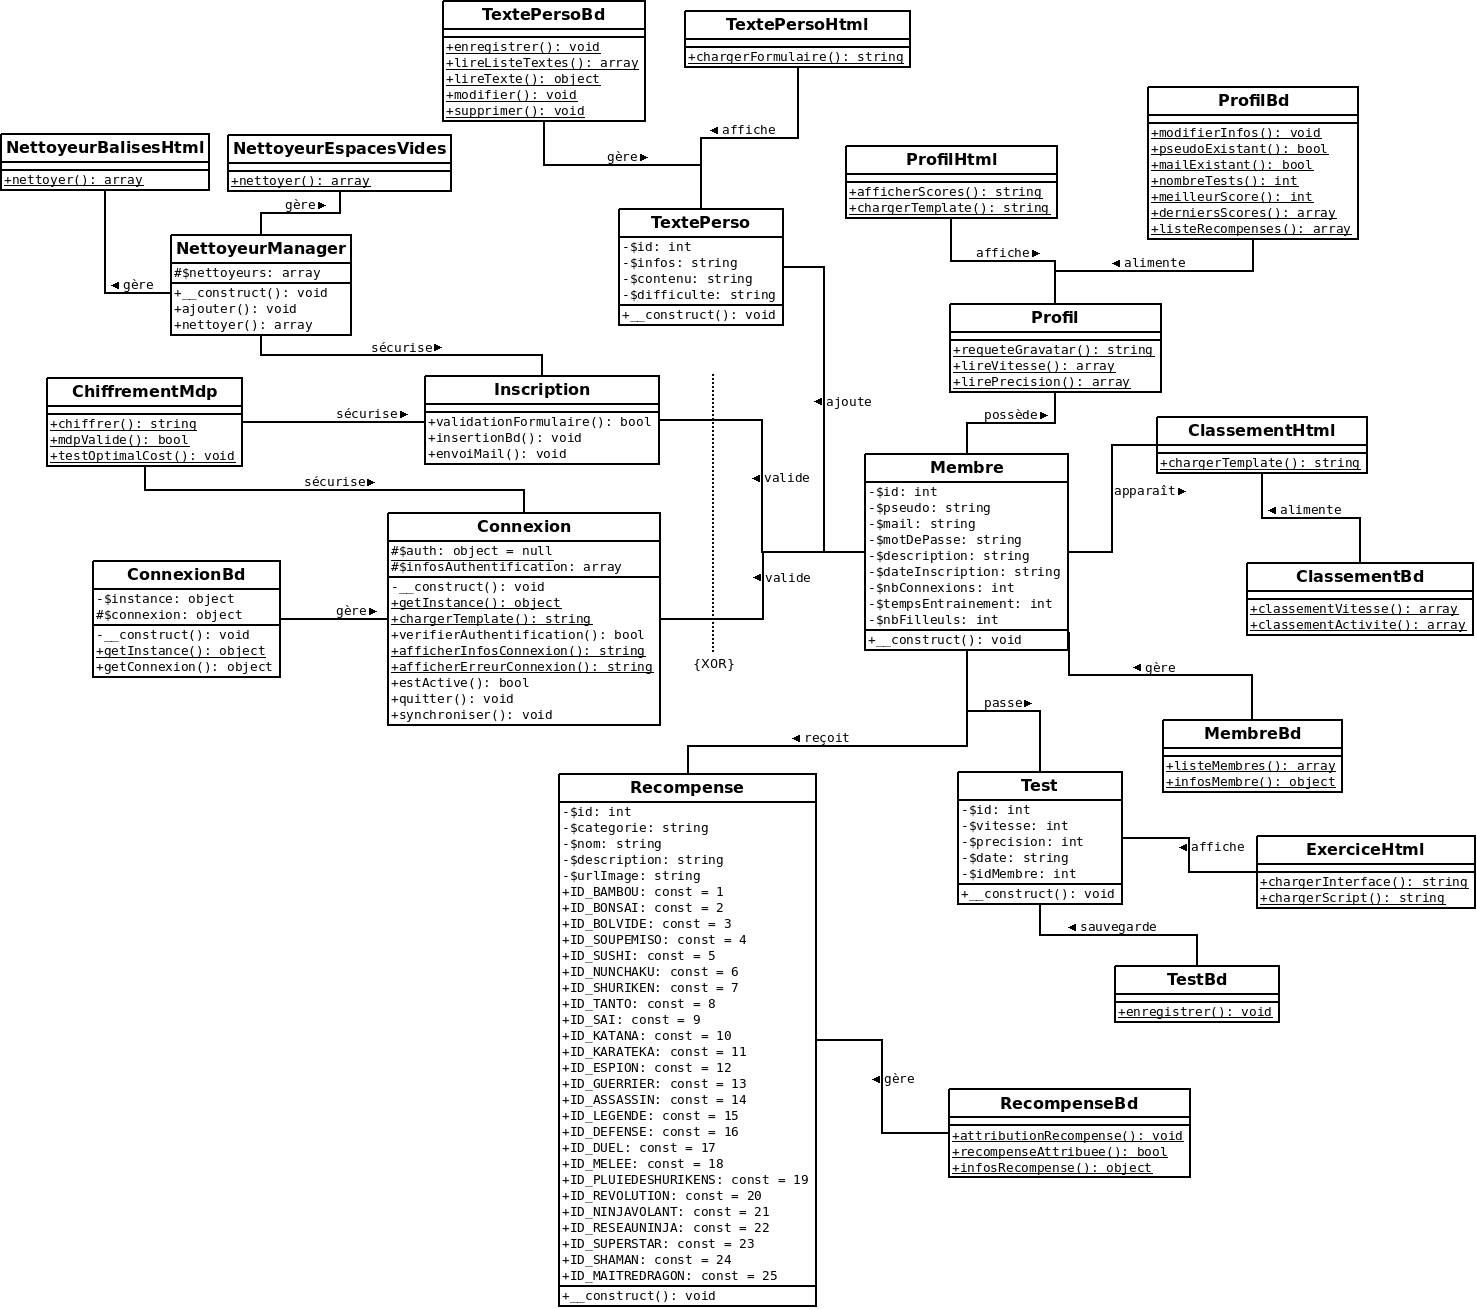
\includegraphics[scale=0.3]{poo.png}
\end{center}
\caption{Schéma UML des classes de Dojoctylo}
\end{figure}

\textbf{N. B.} Les getters, les setters, les paramètres des fonctions, ainsi que les cardinalités n'apparaissent pas sur ce schéma. C'est tout à fait volontaire à des fins de simplification.

Vous noterez par ailleurs que le constructeur est privé à certains endroits (notamment pour les classes \og~ConnexionBd~\fg{} et \og~Connexion~\fg), ceci afin d'implémenter le design pattern Singleton. À noter aussi que \og~ConnexionBd~\fg{} gère la connexion avec MySQL via PDO (PHP Data Objets), tandis que \og~Connexion~\fg{} gère la connexion de l'utilisateur à son compte. Ce sont deux classes très différentes, mais directement liées par la force des choses...

\subsubsection{Sécurité}

Sur Dojoctylo, la sécurité n'a pas été négligée. Tout d'abord, chaque champ de chaque formulaire est soigneusement vérifié, à la fois côté client (en JavaScript) et côté serveur (en PHP). De même, avant soumission d'un formulaire, en plus de la validation, PHP nettoie systématiquement la saisie de l'utilisateur pour éviter une faille XSS (Cross-Site Scripting) et des injections SQL (Structured Query Language). En particulier, la fonction \og~trim~\fg{} est utilisée pour supprimer les espaces inutiles, et la fonction \og~strip\_tags~\fg{} pour supprimer les balises.

Par ailleurs, les mots de passe ne sont évidemment pas stockés en clair dans la base de données. Nous aurions pu utiliser les algorithmes MD5 ou SHA-1 qui ont le mérite d'être extrêmement simples à utiliser, mais ces derniers ne sont hélas pas suffisamment sécurisés. Ce sont en effet des algorithmes qui ont la réputation d'être rapides, et donc facilement cassables pour des pirates avec une puissance de calcul modérée. Ces algorithmes sont particulièrement vulnérables aux attaques par force brute et par dictionnaire, et il est relativement aisé de retrouver le hash MD5 ou SHA-1 d'un mot de passe usuel. Pour toutes ces raisons, Dojoctylo s'appuie sur la fonction \og~password\_hash~\fg{} de PHP pour le hashage des mots de passe. À l'heure actuelle, cette fonction utilise l'algorithme Bcrypt et génère automatiquement un \og~cost~\fg{} (temps de traitement) et un \og~salt~\fg{} (grain de sel) afin de garantir une sécurité maximum.

Finalement, lorsque le programme a besoin de vérifier l'authentification de l'utilisateur, c'est la fonction \og~password\_verify~\fg{} de PHP qui est appelée. Et comme nous sommes en POO, tout cela a été rassemblé dans une classe utilitaire dédiée au chiffrement~!

\begin{lstlisting}
public static function chiffrer($mdp)
{
    $hash = password_hash($mdp, PASSWORD_DEFAULT);
    return $hash;
}

public static function mdpValide($mdp, $hash)
{
    if(password_verify($mdp, $hash)) {
        return true;
    } else {
        return false;
    }
}
\end{lstlisting}


\textbf{N. B.} \og~password\_hash~\fg{} et \og~password\_verify~\fg{} sont de nouvelles fonctions natives, utilisables uniquement en PHP 5.5 et versions ultérieures. Compte tenu du fait que le serveur de la fac exploite encore PHP 5.4, il a fallu utiliser une librairie pour assurer la compatibilité ascendante.

\subsubsection{Gravatar}

Sur Dojoctylo, tout membre peut ajouter une image à son profil. En revanche, il ne s'agit pas d'un ajout traditionnel puisque c'est ici l'image de Gravatar qui est récupérée par le programme via une API (Application Programming Interface).

\begin{lstlisting}
public static function requeteGravatar($auth)
{
    $email = trim($auth->getMail());
    $email = strtolower($email);
    $hash = md5($email);
    $url = "http://www.gravatar.com/avatar/" . $hash . "?s=100";
    return $url;
}
\end{lstlisting}


Conformément à ce qui est expliqué dans la documentation de l'API de Gravatar, il suffit simplement de récupérer l'adresse e-mail du membre en question, de lui faire subir un traitement léger (tout en minuscules et suppression des espaces de début et de fin), puis de créer un hash MD5 à partir de la chaîne de caractères obtenue. Il suffit ensuite de placer l'URL de Gravatar contenant le hash dans un attribut \og~src~\fg{} d'un élément \og~img~\fg, et le tour est joué~! Le paramètre \og~s~\fg{} sert ici à spécifier la taille de l'image attendue.

\newpage

% ==========================================================================
% ==================== IV. Perspectives d'évolution ========================
% ==========================================================================

\part{Perspectives d'évolution}

Dans son état actuel, Dojoctylo est opérationnel. Néanmoins, on peut quand même donner quelques pistes d'amélioration. Nous parlerons donc ici de factorisation et documentation du code, de fonctionnalités sociales, de l'espace d'administration, sans oublier le référencement naturel...

\section{Factorisation et documentation complète du code}

Le code source de Dojoctylo est fonctionnel dans la mesure où il fait ce qu'on lui demande. Cela dit, il serait intéressant d'optimiser celui-ci en intégrant davantage de design patterns pour le style, en utilisant de l'héritage ou des traits pour éviter les redondances, et en documentant l'ensemble avec un outil comme Doxygen.

L'auteur de ces lignes est pour l'instant le seul développeur de Dojoctylo, mais qui sait, ce sera peut-être amené à changer si l'application est publiée et prend de l'ampleur. Dans tous les cas, ne serait-ce que pour simplifier la maintenance de Dojoctylo, avoir un code propre et documenté est judicieux.

\section{Développement des fonctionnalités sociales}

Les fonctionnalités sociales qu'il serait intéressant de développer sur Dojoctylo peuvent être réparties en trois groupes~: réseautage, forum, compétitions en temps réel.

\subsection{Réseautage social}

L'idée ici n'est pas de transformer Dojoctylo en un réseau social complet comme peut l'être Facebook, mais seulement de permettre aux membres de se connecter sur le site en tant qu'amis. Cela permettrait notamment aux membres d'organiser des compétitions privées avec seulement certaines personnes triées sur le volet.

\subsection{Forum}

Le forum serait le lieu où les membres de Dojoctylo pourraient échanger des anecdotes sur la dactylographie, sur les claviers qu'ils utilisent, sur leurs records, etc. Le forum serait un module à part entière du site et serait accessible de facto à toutes les personnes disposant d'un compte sur Dojoctylo.

\subsection{Compétitions en temps réel}

Cette fonctionnalité ambitieuse serait certainement la plus difficile à mettre en place. Il s'agirait ici de créer un module de compétitions en temps réel à l'aide de Node.js et Socket.IO. Les utilisateurs pourraient donc concourir en tapant des textes et voir à tout moment la progression des adversaires, exactement comme dans un jeu multijoueur. Et puisqu'il est bon de ne pas faire les choses à moitié, un tchat pourrait venir agrémenter le module afin que les utilisateurs puissent se parler avant et après chaque \og~round~\fg.

\section{Développement d'un espace d'administration}

À l'heure actuelle, Dojoctylo ne dispose pas d'espace d'administration. Ce n'est certes pas une priorité car il n'y a pour l'instant que l'auteur de ces lignes qui aurait accès à cette interface, mais cela pourrait s'avérer pratique à plus ou moins long terme si de nouvelles personnes venaient à intégrer le projet pour donner un coup de main.

L'espace d'administration permettrait surtout d'ajouter dynamiquement des tutoriels, de suivre les nouvelles inscriptions, et de suspendre des membres irrespectueux ou tricheurs.

\section{Référencement naturel (SEO)}

Si Dojoctylo se voyait un jour publié, il serait de bon ton de procéder à son optimisation complète en interne, de sorte qu'il puisse être correctement indexé et positionné par les moteurs de recherche.

Avant toute chose, il conviendrait d'ajouter du contenu textuel sur plusieurs pages, avec quelques mots-clés bien choisis. Les pages de sélection des modes d'apprentissage, de pratique et de compétition sont, par exemple, assez pauvres en contenu. Or on sait que Google, entre autres, s'appuie beaucoup sur ce contenu pour classer les pages entre elles. Il est donc important de donner quelque chose de consistant à manger aux robots d'indexation si l'on veut être un minimum visible dans les SERPs (Search Engine Results Pages).

En outre, il faudrait faire quelques ajustements du code HTML pour que le site soit réellement \og~SEO-friendly~\fg. Il faudrait d'abord revoir la logique autour du titre \og~h1~\fg{} qui ne contient que \og~Dojoctylo~\fg{} sur toutes les pages. Il faudrait ensuite ajouter une \og~meta description~\fg{} unique sur chacune des pages du site. La balise \og~title~\fg, quant à elle, est déjà optimisée.

Plus technique, mais indispensable~: la réécriture d'URL devrait être implémentée pour éviter le contenu dupliqué, valoriser les mots-clés, et améliorer l'ergonomie en matière de navigation. À ce propos, un fil d'Ariane pourrait aussi être ajouté.

Pour des raisons évidentes, il serait également judicieux d'injecter des métadonnées dans le code source du site pour que les moteurs de recherche comprennent réellement ce qu'il contient. Les microformats ou microdonnées pourraient ici être utilisés afin d'apporter cette dimension sémantique à l'application.

Enfin, il faudrait impérativement optimiser toutes les images (par simple redimensionnement et compression sans perte) car le site est pour l'instant très lourd, d'où une vitesse de chargement relativement lente. Or en plus d'affecter négativement les performances du site, le surpoids des images risque de faire fuir les utilisateurs pressés, et donc d'augmenter le taux de rebond.

Et pour ce qui est du netlinking, c'est déjà une autre histoire...

\newpage

% ==========================================================================
% =============================== Conclusion ===============================
% ==========================================================================

\part*{Conclusion}

En seulement quelques semaines de travail, Dojoctylo est déjà un site web fonctionnel. Bien sûr, il reste des choses à faire, mais les stories du backlog réellement essentielles pour le projet ont été implémentées.

Pour l'instant, Dojoctylo n'est qu'un projet universitaire qui s'est avéré particulièrement intéressant pour mettre en pratique les enseignements vus en cours. De nombreuses compétences acquises ou consolidées tout au long de cette année ont pu être mobilisées, que ce soit HTML, CSS, JavaScript, Ajax, PHP orienté objet, MySQL, UML, et bien d'autres choses encore...

À terme, Dojoctylo deviendra certainement un terrain de jeu propice à l'expérimentation en matière de développement. L'idée est bien sûr d'apprendre par la pratique en appliquant des notions abstraites à des cas concrets. Dojoctylo se verra certainement enrichi de nombreuses autres fonctionnalités, comme on a pu le voir dans la dernière partie de ce rapport. In fine, il y a de grandes chances que ce site soit publié pour que les internautes puissent en profiter.

Dojoctylo~: le site qui va faire de vous un ninja du clavier~!

\end{document}          
